
\documentclass{beamer}

% There are many different themes available for Beamer. A comprehensive
% list with examples is given here:
% http://deic.uab.es/~iblanes/beamer_gallery/index_by_theme.html
% You can uncomment the themes below if you would like to use a different
% one:
%\usetheme{AnnArbor}
%\usetheme{Antibes}
%\usetheme{Bergen}
%\usetheme{Berkeley}
%\usetheme{Berlin}
%\usetheme{Boadilla}
%\usetheme{boxes}
%\usetheme{CambridgeUS}
%\usetheme{Copenhagen}
%\usetheme{Darmstadt}
%\usetheme{default}
%\usetheme{Frankfurt}
%\usetheme{Goettingen}
%\usetheme{Hannover}
%\usetheme{Ilmenau}
%\usetheme{JuanLesPins}
%\usetheme{Luebeck}
%\usetheme{Madrid}
%\usetheme{Malmoe}
\usetheme{Marburg}
%\usetheme{Montpellier}
%\usetheme{PaloAlto}
%\usetheme{Pittsburgh}
%\usetheme{Rochester}
%\usetheme{Singapore}
%\usetheme{Szeged}
%\usetheme{Warsaw}



\title{Exploration vs. Exploitation}

% A subtitle is optional and this may be deleted
%\subtitle{Optional Subtitle}

\author{Krishna Devkota}
% - Give the names in the same order as the appear in the paper.
% - Use the \inst{?} command only if the authors have different
%   affiliation.

\institute[Universities of Somewhere and Elsewhere] % (optional, but mostly needed)
{
  %
  
  Bielefeld University\\
  5th May 2017
}
% - Use the \inst command only if there are several affiliations.
% - Keep it simple, no one is interested in your street address.

\date{Reinforcement Learning in Autonomous Social agents}
% - Either use conference name or its abbreviation.
% - Not really informative to the audience, more for people (including
%   yourself) who are reading the slides online

\subject{Computer Science}
% This is only inserted into the PDF information catalog. Can be left
% out. 

% If you have a file called "university-logo-filename.xxx", where xxx
% is a graphic format that can be processed by latex or pdflatex,
% resp., then you can add a logo as follows:

% \pgfdeclareimage[height=0.5cm]{university-logo}{university-logo-filename}
% \logo{\pgfuseimage{university-logo}}

% Delete this, if you do not want the table of contents to pop up at
% the beginning of each subsection:
\AtBeginSubsection[]
{
  \begin{frame}<beamer>{Outline}
    \tableofcontents[currentsection,currentsubsection]
  \end{frame}
}

% Let's get started
\begin{document}

\begin{frame}
  \titlepage
\end{frame}

\begin{frame}{Outline}
  \tableofcontents
  % You might wish to add the option [pausesections]
\end{frame}

% Section and subsections will appear in the presentation overview
% and table of contents.
\section{Overview}

\begin{frame}{The Exploration vs. Exploitation dilemma}


$\blacksquare$ Important aspect of model-free algorithms is a need for exploration\\
$\blacksquare$ As model unknown, learner needs to try out different actions to see their results\\
$\blacksquare$ How can a RL agent balance Exploration vs. Exploitation?

\hspace{5mm}\textcolor{blue}{\textit{One of the fundamental questions in RL}}

\vspace{4mm}
  \begin{itemize}
  \color{blue}
  \item {Exploration}\\
  \textcolor{black} {Gather more information}
  \item {
    Exploitation\\
    \textcolor{black}{Make the best decision given current information}
  }
  \end{itemize}
  \vspace{4mm}
  $\blacksquare$ Sometimes, immediate sacrifices might lead to better long-term strategies
\end{frame}



\begin{frame}{Exploration vs. Exploitation (In Practice)}

\vspace{3mm}
  \begin{itemize}
  \color{blue}
  
  \item {Restaurant Selection}\\
  \textcolor{black} {Exploitation: Go to a Restaurant that you know well}\\
  \textcolor{black} {Exploration: Try a new restaurant}
  
  \item {Playing a game}\\
    \textcolor{black}{Exploitation: Play a move that you are confident of}\\
    \textcolor{black}{Exploration: Try a new move that you haven't played much}
    
  \item {Advertisement}\\
    \textcolor{black}{Exploitation: Play an advertisement that has been received well}\\
    \textcolor{black}{Exploration: Try a new Ad that has not been played yet}
 
  \end{itemize}  
\end{frame}

\begin{frame}{Quick Recap of Markov Decision Process (MDP)}
Markov decision processes formally describe an environment for reinforcement learning (decision making)



\begin{itemize}
\item{A MDP can be represented as a 4-tuple $\langle S,A,P,R \rangle$ where:}

\begin{figure}
\flushright
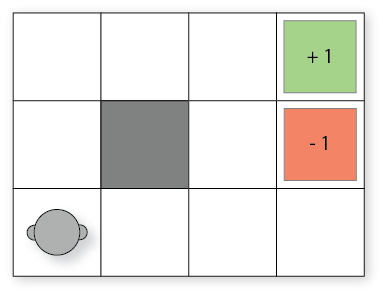
\includegraphics[width=3cm]{Enviroment_MDP}
\end{figure}

\item{S is a set of states}
\item{A is set of all the actions that the agent can take}
\item{$P(s'|s,a)$ is a function that defines the transition probability \textit{(Markovian)}}
\item{$R(s,a)$ is the reward function, which gives the probability of receiving reward r after choosing a in state s }

\end{itemize}

\end{frame}

\begin{frame}{Three different classes of approach to the problem}
\begin{itemize}
\item{Random exploration}
    \begin{itemize}
    \item{Explore random actions (e.g. $\epsilon-greedy$, softmax)}
    \end{itemize}
\item{Optimism in the face of uncertainty}
    \begin{itemize}
    \item{estimate uncertainty on value}
    \item{Prefer to explore states/actions with highest uncertainty}
    \end{itemize}
\item{Information state space}
    \begin{itemize}
    \item{Consider agent's information as part of its state}
    \item{Look ahead to see how information helps reward}
    \end{itemize}
\end{itemize}  
  
  
  
\end{frame}






\section{Random exploration (naive approach)}

\begin{frame}{Random exploration (naive approach)}


\textcolor{blue}{Multi-armed Bandit Problem (single-state MDP)}

One of the simplest way to model a exploration/ exploitation dilemma is using a multi-armed Bandit Problem
 
\begin{figure}
\centering
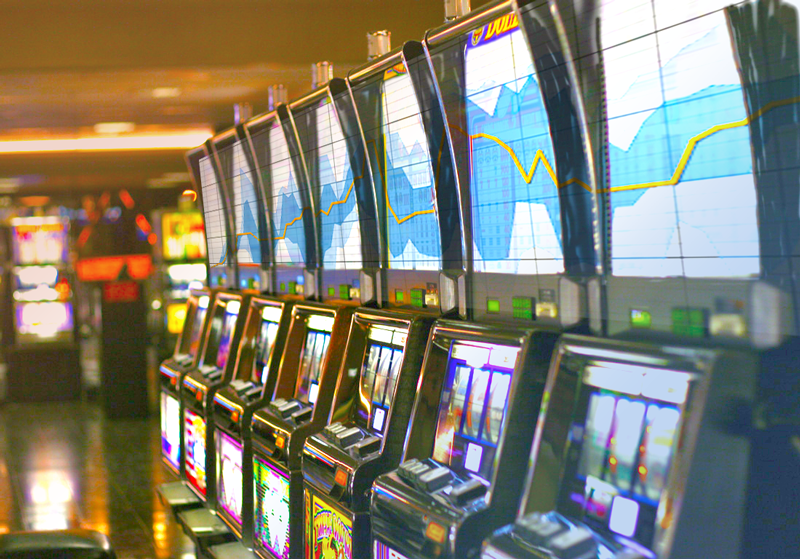
\includegraphics[width=5cm]{bandit}
\caption{Bandit Machines}
\end{figure} 

\end{frame}

\begin{frame}
\textcolor{blue}{Multi-armed bandit problem}

\begin{itemize}

\item{models the exploration/exploitation trade-off inherent in sequential
decision problems}

\item{a sequential experiment with the goal of achieving the largest possible reward from a payoff distribution}

\item{Parameters of payoff distribution unknown}

\item{ Choice involves a fundamental trade-off between:}
\begin{itemize}
\item{the utility gain from exploiting arms that appear to be doing well (based on limited sample
information)}
\item{\textit{vs.} exploring arms that might potentially be optimal, but which appear to be inferior
because of sampling variability}
\end{itemize}
\item{sometimes referred to as 'earn vs learn'}

\end{itemize}

\end{frame}


\begin{frame}{Formalizing Multi-armed Bandit problem}

\begin{itemize}
    
  \item {Can be represented as a Tuple $\langle A, R \rangle$}\\
  
  
  \item {A is known set of Arms that can be Pulled i.e. actions that can be taken (m)}\\
    
    
  \item {$R^a(r) = \mathcal{P}[r|a]$ is the unknown Probability distribution over rewards}\\
  
  \item {Action taken at each step t by the agent : $a_t \in A$}\\
  
  \item {Reward generated by the environment: $r_t \sim R^{a_t}$}\\
    
\end{itemize}  
 $\blacksquare$ Goal : maximize cumulative reward $$\sum_{\tau=1}^{t} r_\tau$$

\end{frame}

\begin{frame}{Regret}

\begin{itemize} 
  \item {\textcolor{blue}{Action-value}}\\
  mean reward for action a, $Q(a) = E[r|a]$
  
  \item {\textcolor{blue}{Optimal value ($V^*$)}}\\
  $V^* = Q(a^*) = max_{a \in A} Q(a)$
    
  \item {\textcolor{blue}{Regret}}\\
  Opportunity lost for each step
  $l_t = E[V^* - Q(a_t)]$
  
  \item {\textcolor{blue}{Total Regret}}\\
  Opportunity lost over all the steps
  
  $L_t = E \big[ \sum_{\tau=1}^{t}(V^* - Q(a_\tau))\big]$
  
\end{itemize}  
$\blacksquare$ Goal : maximize cumulative reward, hence minimize total regret
\end{frame}

\begin{frame}{Regret as counts and gaps}

\begin{itemize} 
  \item {\textcolor{blue}{Count ($N_t(a)$)}}\\
  Expected number of times an action is taken, 
  
  \item {\textcolor{blue}{Gap ($\bigtriangleup_a$)}}\\
  Difference in value between action (a) and optimal action ($a^*$)
  $\bigtriangleup_a = V^* - Q(a)$
    
  \item {\textcolor{blue}{Regret as a function of count and gap}}\\
    
  $L_t = \sum_{a \in A} E \big[ N_t(a)\big]\bigtriangleup_a $
  
\end{itemize}  
$\blacksquare$ Goal : Find a good algorithm, so we visit the less desired state, the least amount of times i.e. small counts for large gaps\\
$\blacksquare$ Problem : we don't know the optimal value ($V^*$), and hence the gaps
\end{frame}

\begin{frame}{Regret}
\begin{figure}
\centering
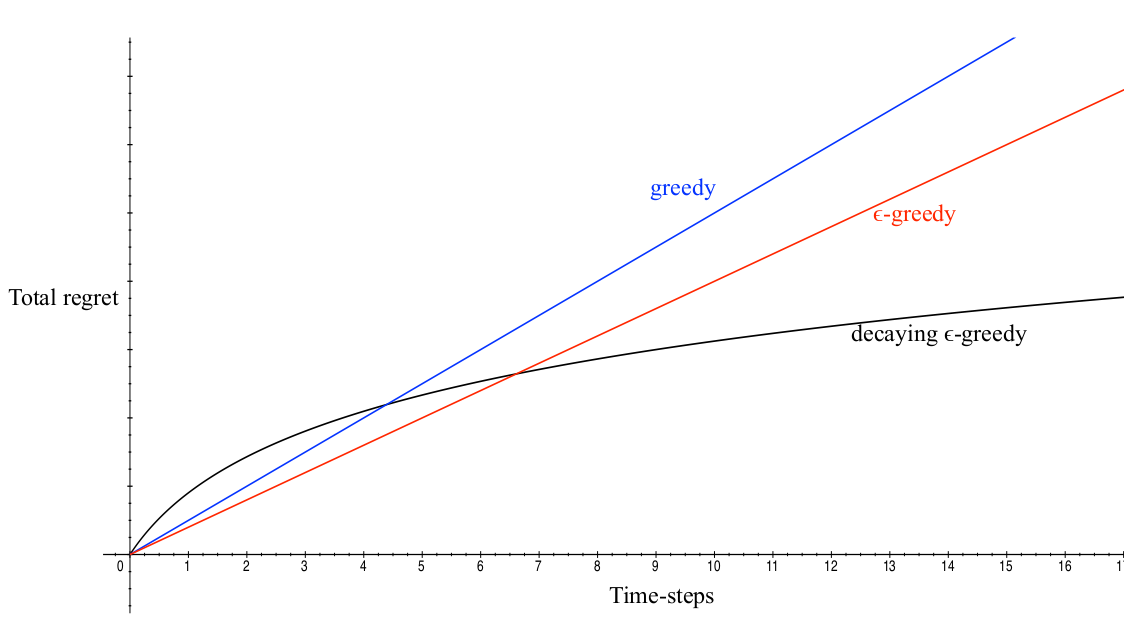
\includegraphics[width=5cm]{regret_curve}
\caption{Comparing Regret values for different naive-algorithms}
\end{figure}   
\begin{itemize}
\item{If an algorithm \textcolor{blue}{forever explores}, it will have a linear regret ($\epsilon-greedy$)}
\item{If an algorithm \textcolor{blue}{never explores}, it will have a linear regret (greedy)}
\item{So, how do we achieve sub-linear total regret?}

\end{itemize}

 
\end{frame}

\begin{frame}{A quick look at Greedy algorithm}
\begin{figure}
\centering
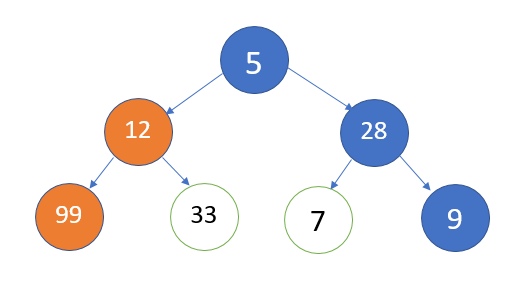
\includegraphics[width=2.5cm]{greedy}
\caption{Greedy algorithm based on local optimum}
\end{figure} 
\begin{itemize} 
  \item {Consider algorithm that estimates $\hat{Q_t}(a)$ which is closest to $Q_t(a)$ i.e. the \textcolor{blue}{MC evaluation}: 
  $$\hat{Q_t(a)} = \frac{1}{N_t(a)}\sum_{t=1}^{T}r_t1(a_t = a)$$ }
    
  \item { Using \textcolor{blue}{greedy algorithm} gives us:
  ${a_t}^* = argmax_{a \in A} \hat{Q_t}(a)$}
  
  \item {\textcolor{blue}{Problem}}: We might get stuck onto a suboptimal action again and again
\end{itemize}

\end{frame}

\subsection{$ \epsilon greedy $ }

\begin{frame}{The $ \epsilon - greedy $ algorithm }

\begin{figure}
\centering
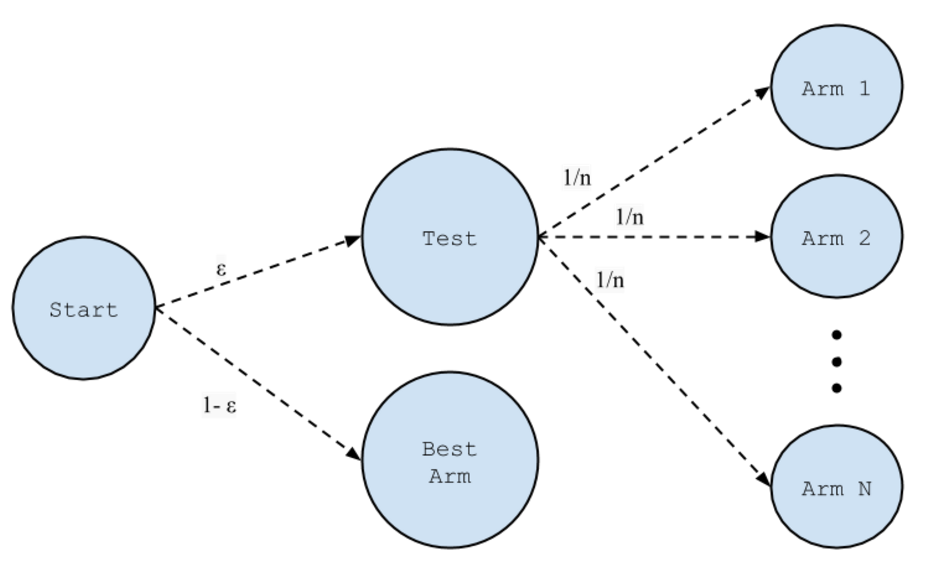
\includegraphics[width=4cm]{egreedytree}
\end{figure} 

  \begin{itemize}
  \item {Using the $ \epsilon - greedy $ algorithm, we want to introduce some randomness into our greedy approach }
  \item {How do we do that??}
  \begin{itemize}
  \item{with probability $1-\epsilon$ act greedily, i.e. select ${a_t}^* = argmax_{a \in A} \hat{Q_t}(a)$}
  \item{with probability $\epsilon$, select a random action}
  \end{itemize}    
  \end{itemize}
  \end{frame}
  
  \begin{frame}
  

  
  
  \textcolor{blue}{Advantages of $\epsilon - greedy$ exploration:}
  \begin{itemize}
  \item {Simplest idea for ensuring continual exploration}
  \item{All m-actions are tried with non-zero probability}
  
  \end{itemize}
  \textcolor{blue}{Drawback of $\epsilon - greedy$ exploration:}
  \begin{itemize}
  \item {Random actions selected uniformly. The worst possible action is just as likely to be selected as the second best action}
    
  \end{itemize}
\end{frame}


\subsection{Softmax}

\begin{frame}{Softmax }

We saw that the $\epsilon-greedy$ selected the random actions uniformly, giving equal weights to the good and the bad

Softmax remedies this by assigning a rank or weight to each of the actions, according to their action-value estimate.
  \begin{itemize}
  \item {Bias exploration towards promising actions}
  \item{Softmax action selection methods grade action probabilities by estimated values}
  \item{The most common softmax uses a Gibbs (or Boltzmann) distribution}
  \end{itemize}


\textcolor{blue}{Advantages:}
\begin{itemize}
 \item{As appropriate weight associated with each action, the worst actions are unlikely to be chosen}
 
 \item{Good in scenarios where the worst actions are very unfavourable}
 \end{itemize}
\end{frame}


\begin{frame}{Softmax}

******************** Mathematical formulation *********************

\end{frame}




\subsection{Optimistic Initialization}

\begin{frame}{Optimistic Initialization}
  \begin{itemize}
  \item {initialize Q(a) to high value (i.e. assume all of our actions pay the best possible}
  $$ Q(a) = r_{max} $$
  
  
  
  \item {Use MC evaluation to incrementally update action value}
  
  \item{$\hat{Q_t}(a_t) = \hat{Q}_{t-1} +\frac{1}{N_t(a_t)}(r_t-\hat{Q}_{t-1})$}
  \end{itemize}

\textcolor{blue}{Advantage:}
  \begin{itemize}
  \item {Encourages exploration of unknown values}
  
  \end{itemize}
  \textcolor{blue}{Drawback:}
  \begin{itemize}
  \item{We need to know the maximum possible reward $r_{max}$}
  \item {Can still get caught in suboptimal action}
  \end{itemize}  
\end{frame}

\begin{frame}{Comparing greedy, $\epsilon$-greedy, and Optimistic Initialization}

For a 10-armed testbed, N = 10 possible actions, 1000 plays\\
Q(a) are chosen randomly from a Normal distribution $N(0,1)$
\begin{figure}
\centering
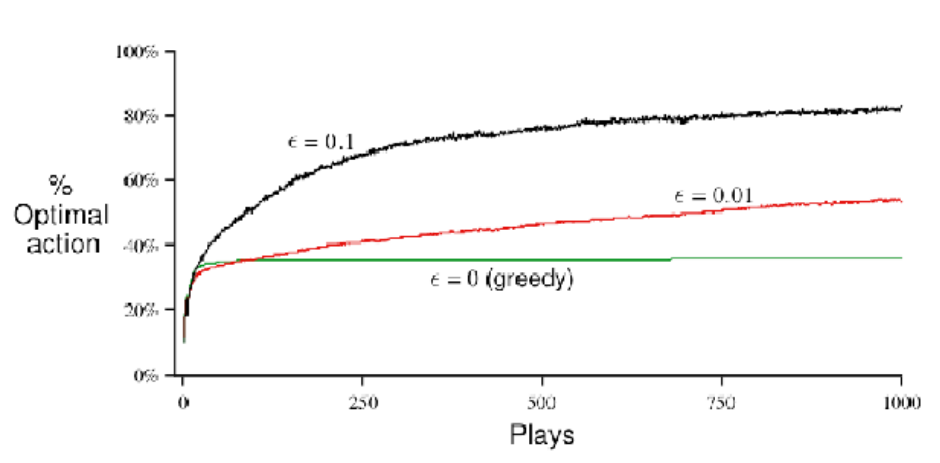
\includegraphics[width=4cm]{Greedy_e_greedy}
\caption{Greedy vs. $\epsilon$-greedy}
\end{figure} 

\begin{figure}
\centering
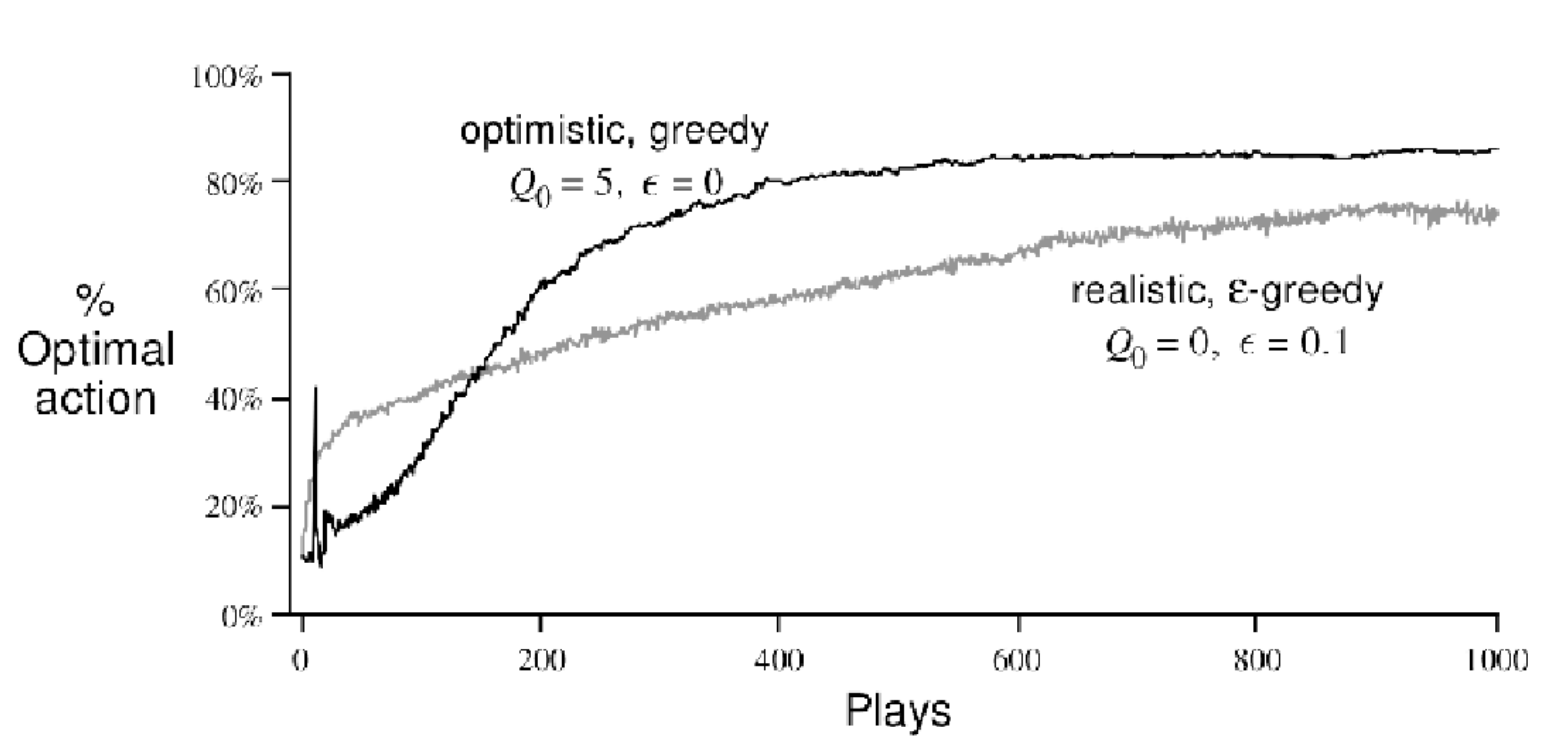
\includegraphics[width=4cm]{optimistic_greedy}
\caption{Normal case vs. Optimistically initialized case}
\end{figure} 


\end{frame}

\section{Methods based on Upper Confidence Bounds (UCBs) } %Optimism in the face of uncertainty

\begin{frame}{Methods based on Upper Confidence Bounds (UCBs) }
\textcolor{blue}{Acting Optimistically in Uncertain situations}

\begin{figure}
\centering
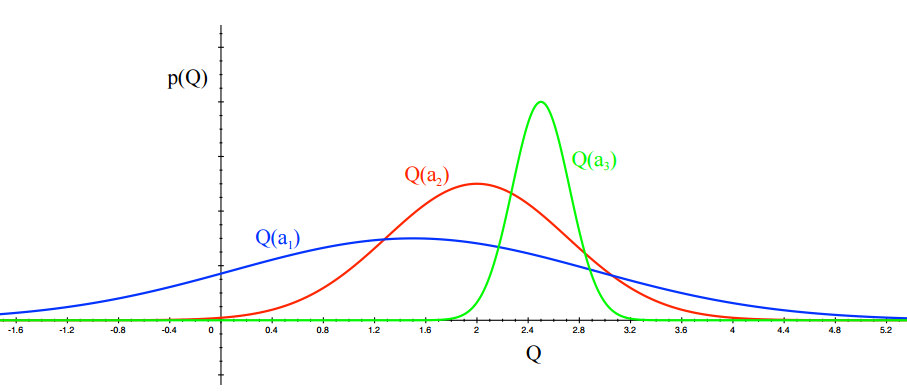
\includegraphics[width=7cm]{Optimism_curves}
\end{figure}

\begin{itemize}
 \item{The more uncertain we are about an action value}
 \item{The more important it is to explore that action}
 \item{It could turn out to be the best action}
\end{itemize}    
\end{frame}

\subsection{Upper Confidence Bounds}

\begin{frame}{Methods based on Upper Confidence Bounds (UCBs) }
\begin{itemize}
\item{So, far we've talked about estimating the mean (when we talk about Q-values)}
\item{i.e. which arm gives the max reward on average}
\item{but we don't know the uncertainty in each arm}
\item{the range of values that the arm can give}
\end{itemize}

$\blacksquare$ We can assume two different approaches to address this
\begin{itemize}
\item{\textcolor{blue}{Frequentist:}}\\
where we assume nothing about the distribution
\item{\textcolor{blue}{Bayesian:}}\\
assume we have some prior probabilities over the Q-values
\end{itemize}

  
\end{frame}







\begin{frame}{Methods based on Upper Confidence Bounds (UCBs) }
\begin{itemize}
  \item{\textcolor{blue}{Confidence interval}}\\
  a range of values within which we are sure the mean lies with a certain probability
    
  \item{For an action which has been tried less often, our estimated reward is less accurate so the confidence interval is larger} 
  \item{It shrinks as we get
more information (i.e. try the action more often)}

  \item{So, instead of trying the action with the highest mean, we can try
the action with the highest upper bound on its confidence interval}
\item{This is known as an optimistic policy}
\end{itemize}
\end{frame}


\begin{frame}{Methods based on Upper Confidence Bounds (UCBs) }
\textcolor{blue}{Steps:}\\
\begin{itemize}

\item{For each action value, estimate an upper confidence $\hat{U}_t(a)$ such that:}\\
$Q(a) \leq \hat{Q}_t(a) + \hat{U}_t(a)$ with high probability

\item{determined by the number of times N(a) has been selected}
\begin{itemize}
\item{Small $N_t(a) \Rightarrow large \hat{U}_t(a)$}\\
estimated value is uncertain
\item{Large $N_t(a) \Rightarrow small \hat{U}_t(a)$}\\
estimated value is accurate
\end{itemize}
\item{Select action that maximizes the UCB}\\
$a_t = argmax_{a \in A}\hat{Q}_t(a)+\hat{U}_t(a)$
\end{itemize}
\end{frame}

\begin{frame}{Methods based on Upper Confidence Bounds (UCBs) }
\begin{itemize}
  \item{To solve for the bounds, we can turn to: \textcolor{blue}{Chernoff-Hoeffding bound}}
  \item{Then, pick a probability p for the true value to exceed the UCB}
  \item{Solve for $U_t(a)$, and reducing probability p, as more rewards are observed}
  \item{As $t \rightarrow \infty$, we select optimal action as given by:}\\
  $$U_t(a) = \sqrt{\frac{2 log t}{N_t(a)}}$$
\end{itemize} 

This gives us the UCB1 algorithm:
$$ a_t = argmax_{a \in A}Q(a) + \sqrt{\frac{2 log t}{N_t(a)}} $$

\end{frame}

\begin{frame}
\textcolor{blue}{Quick recap of methods based on UCB}
\begin{itemize}
\item{Each arm is assigned an UCB for its mean reward}
\item{Arm with the largest bound to be played}
\item{Bound is not conventional upper limit for a confidence interval, hence difficult to compute}

\item{However, making some basic assumptions, the expected number of times suboptimal arm a would be played by time t is:}\\
$E(n_{at}) \leq \big(\frac{1}{K(a,a^*)}+o(1)\big)log t$\\
where $K(a,a^*)$ is the Kullback-Leibler divergence between the reward distributions for arm $a$ and optimal arm $a^*$
\item{This bound essentially says that the optimal arm will be played exponentially more often than any of the suboptimal arms, for large t}
\end{itemize}
  
\end{frame}


\begin{frame}
  \textcolor{blue}{How do we exploit prior knowledge about rewards?}
  
  \begin{itemize}
  \item{Recall, we started by a unknown distribution over our action-value function}
  \item{Instead, say we start with some distribution over the action value function}
  \item{Let $p[Q|w]$ be some distribution over action-value function, where w is the parameter}
  \item{The parameters w could be (say) the mean and the variances of each of our arms}
  \item{We could then compute posterior distribution over w by using the Bayesian methods}\\
  $p[w|R_1,....,R_t]$
  
  \end{itemize}
  
\end{frame}


\begin{frame}
\begin{itemize}
\item{the posterior can then be used to guide exploration i.e. UCB, and Probability matching}
\item{the performance is better if our knowledge of the prior is accurate}
\end{itemize}

\textcolor{blue}{Random Probability Matching}
    \begin{itemize}
    \item{Randomized probability matching combines many positive aspects of the heuristic strategies mentioned above}
  
  \item{Probability matching selects action a according to probability that a is the optimal action}\\
  $\pi(a|h_t) = P[Q(a)>Q(a'),\forall a' \neq a | h_t]$
  \item{Uncertain actions have higher probability of being max}
  \item{Can be difficult to compute analytically from posterior}   
  \end{itemize}  
\end{frame}

\subsection{Thompson sampling}

\begin{frame}
\textcolor{blue}{Thompson sampling}
  \begin{itemize}
  \item{way to implement probability matching}\\
  $\pi(a|h_t) = P[Q(a)>Q(a'),\forall a' \neq a | h_t]$\\
  $=E_{R|h_t}\big[1(a = argmax_{a \in A}Q(a))\big]$
  \item{Use Bayes law to compute posterior distribution $p[R | h_t]$, where $h_t = a_1,r_1,...,a_{t-1},r_{t-1}$ is the history}
  \item{Sample a reward distribution R from posterior}
  \item{Compute action-value function $Q(a) = E[R_a]$}
  \item{Select action maximising value on sample, $ a_t = argmax_{a \in A}Q(a) $}
  
  \end{itemize}
  
\end{frame}
\begin{frame}
  \textcolor{blue}{Advantages of Probability matching techniques:}\\
  \begin{itemize}
  \item{the tuning parameters, and the decay schedule evolves in a principled, data-determined way}
  \item{In other methods, the parameters are arbitrarily set by analyst, and incorrect values bear huge costs}
  \end{itemize}
  \textcolor{blue}{Disavantages of Probability matching techniques:}\\
  \begin{itemize}
  \item{There is a need to sample from the posterior distribution}
  \item{This can require substantially more computing than other heuristics}
  \end{itemize}
  
\end{frame}




\section{Information State Space}

\subsection{Gittins indices}

\subsection{Bayes- adaptive MDPs}












% Placing a * after \section means it will not show in the
% outline or table of contents.
\section*{Summary}

\begin{frame}{Summary}

$\blacksquare$ We saw how the problem of exploration/ exploitation can be tricky sometimes\\
$\blacksquare$ We looked at some of the heuristic strategies to handle the dilemma (naive)
\begin{itemize}
\item{Equal allocation}
\item{Play-the-winner}
\item{Deterministic greedy strategies}
\item{Hybrid strategies such as $\epsilon-greedy$, and Softmax}
\end{itemize}
$\blacksquare$ We looked at some strategies based on upper bounds
\begin{itemize}
\item{UCB1}
\item{Random Probability matching}
\end{itemize}




  **************Summary goes here***************
\end{frame}



% All of the following is optional and typically not needed. 
\appendix
\section<presentation>*{\appendixname}
\subsection<presentation>*{For Further Reading}

\begin{frame}[allowframebreaks]
  \frametitle<presentation>{For Further Reading}
    
  \begin{thebibliography}{10}
    
  \beamertemplatebookbibitems
  % Start with overview books.

  \bibitem{Author1990}
    A.~Author.
    \newblock {\em Handbook of Everything}.
    \newblock Some Press, 1990.
 
    
  \beamertemplatearticlebibitems
  % Followed by interesting articles. Keep the list short. 

  \bibitem{Someone2000}
    S.~Someone.
    \newblock On this and that.
    \newblock {\em Journal of This and That}, 2(1):50--100,
    2000.
  \end{thebibliography}
\end{frame}

\end{document}


